% Auto-generated by experiments/plot_scaled_derivative_families.py.
% Requires \usepackage{pgfplots} and \pgfplotsset{compat=1.18}.
% Figure label suggestion: \label{fig:scaled-exit-bicycle}
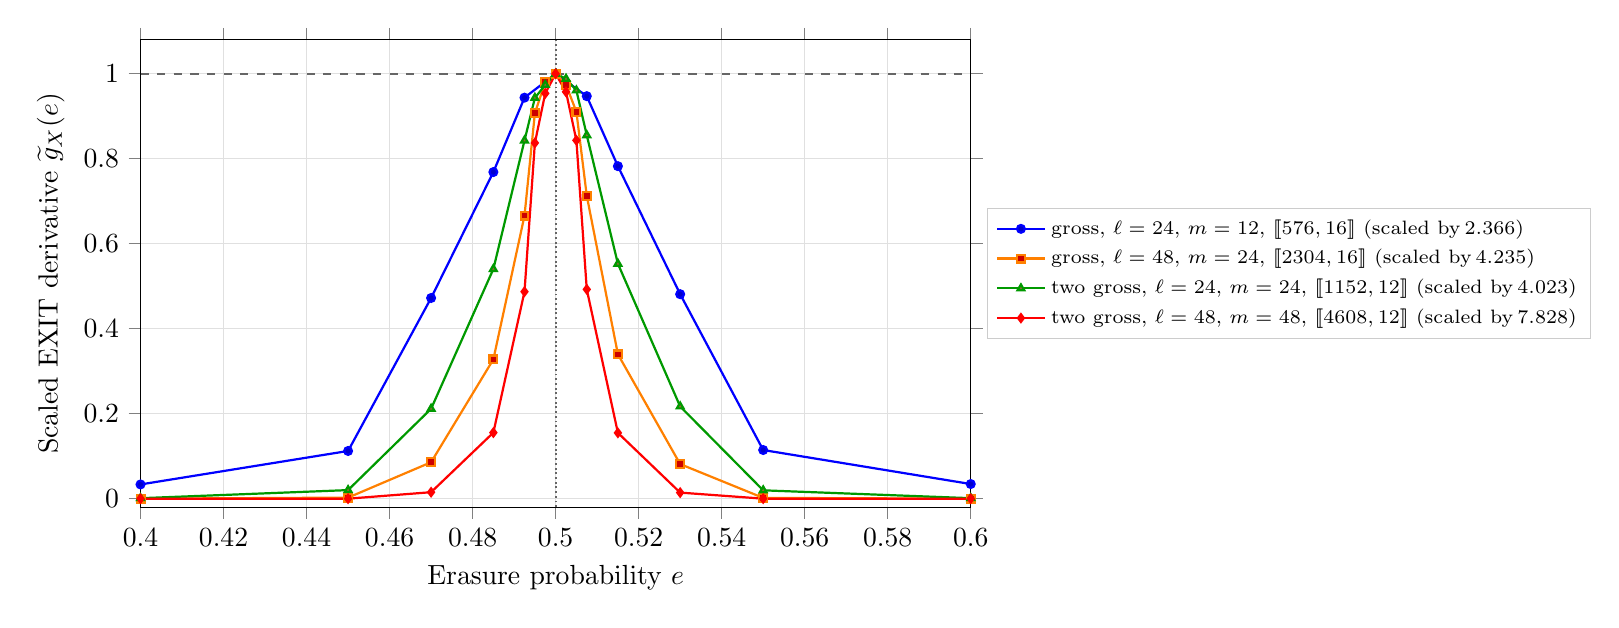
\begin{tikzpicture}
\begin{axis}[
  name=scaledEXITBicycleAxis,
  width=\linewidth,
  height=0.62\linewidth,
  xlabel={Erasure probability $e$},
  ylabel={Scaled EXIT derivative $\widetilde g_X(e)$},
  xmin=0.4, xmax=0.6,
  ymin=-0.02, ymax=1.08,
  grid=both,
  major grid style={black!12},
  minor grid style={black!6},
  tick align=outside,
  legend cell align={left},
  legend style={draw=black!20, fill=white, at={(1.02,0.5)}, anchor=west, font=\scriptsize},
]
\addplot[black!60, densely dotted, line width=0.7pt, forget plot] coordinates {(0.5,-0.02) (0.5,1.08)};
\addplot[black!60, dashed, line width=0.7pt, forget plot] coordinates {(0.4,1) (0.6,1)};
\addplot+[color=blue, mark=*, mark size=1.4pt, line width=0.8pt]
coordinates {(0.4,0.0334921939195) (0.45,0.112254959502) (0.47,0.472262002582) (0.485,0.768666118872) (0.4925,0.943714050945) (0.5,1) (0.5075,0.947247329499) (0.515,0.782507075687) (0.53,0.481230191337) (0.55,0.114485268224) (0.6,0.0344289235826)};
\addlegendentry{gross, $\ell=24$, $m=12$, $\left[\!\left[576,16\right]\!\right]$ ($\mathrm{scaled\ by}\,2.366$)}
\addplot+[color=orange, mark=square*, mark size=1.4pt, line width=0.8pt]
coordinates {(0.4,7.35240055878e-06) (0.45,0.00245780247251) (0.47,0.0857605008035) (0.485,0.32785171025) (0.4925,0.665943680612) (0.495,0.907065656937) (0.4975,0.980442614514) (0.5,1) (0.5025,0.973825454011) (0.505,0.910447761194) (0.5075,0.712925520182) (0.515,0.339811615159) (0.53,0.0813490604682) (0.55,0.00182234499564) (0.6,7.35240055878e-06)};
\addlegendentry{gross, $\ell=48$, $m=24$, $\left[\!\left[2304,16\right]\!\right]$ ($\mathrm{scaled\ by}\,4.235$)}
\addplot+[color=green!60!black, mark=triangle*, mark size=1.4pt, line width=0.8pt]
coordinates {(0.4,0.00110350607627) (0.45,0.0201544509409) (0.47,0.211541915271) (0.485,0.540454129224) (0.4925,0.842855147367) (0.495,0.943148484425) (0.4975,0.973739349071) (0.5,1) (0.5025,0.98826651767) (0.505,0.96074870792) (0.5075,0.855356893421) (0.515,0.5529015536) (0.53,0.2170295133) (0.55,0.0196356234909) (0.6,0.00115937980165)};
\addlegendentry{two gross, $\ell=24$, $m=24$, $\left[\!\left[1152,12\right]\!\right]$ ($\mathrm{scaled\ by}\,4.023$)}
\addplot+[color=red, mark=diamond*, mark size=1.4pt, line width=0.8pt]
coordinates {(0.4,0) (0.45,4.85380344038e-06) (0.47,0.015221527589) (0.485,0.155431729637) (0.4925,0.487190812721) (0.495,0.837184017396) (0.4975,0.953859744496) (0.5,1) (0.5025,0.9573933134) (0.505,0.843367762979) (0.5075,0.492525142702) (0.515,0.154903204373) (0.53,0.0142798897216) (0.55,4.85380344038e-06) (0.6,0)};
\addlegendentry{two gross, $\ell=48$, $m=48$, $\left[\!\left[4608,12\right]\!\right]$ ($\mathrm{scaled\ by}\,7.828$)}
\end{axis}
\end{tikzpicture}
